\documentclass[border=0pt]{standalone}
\usepackage{tikz}
\usetikzlibrary{arrows,shapes.geometric}
\usepackage{xifthen} % cnttest
\begin{document}

%%% 2D staggered grid picture from StagYY Users' Manual
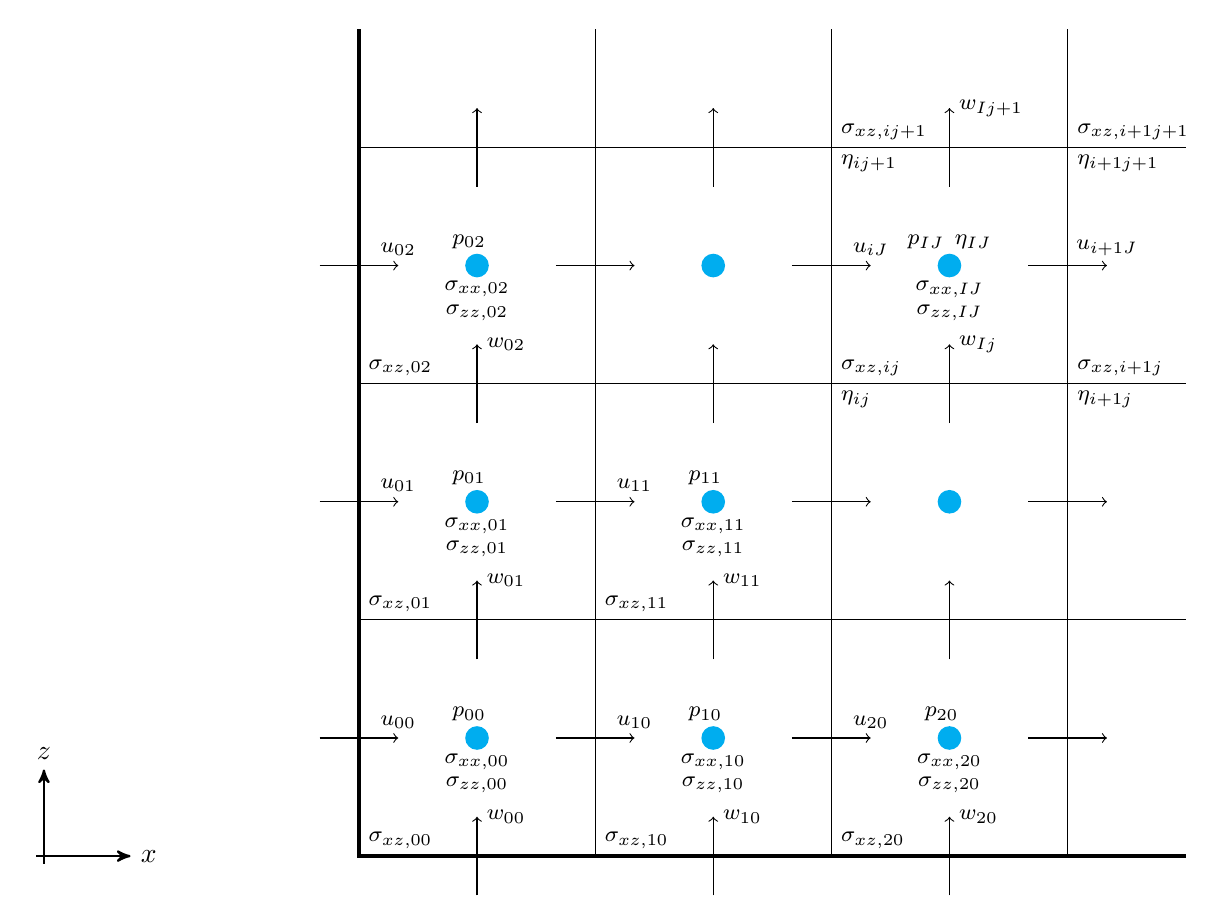
\begin{tikzpicture}[
every node/.style={color=black},
axis/.style={thick, ->, >=stealth'}
]
% small coordinate system
\draw[axis] (-0.1,0)  -- (1.1,0) node(xline)[right]{$x$};
\draw[axis] (0,-0.1) -- (0,1.1) node(yline)[above] {$z$};
% larger grid w/ points etc.
% grid
\draw[very thick] (14.5,0) -- (4,0) -- (4,10.5);
% horizontal arrows 
\foreach \i in {0,...,3}{
\foreach \j in {0,1,2}{
\draw[->] (3.5+3*\i,1.5+3*\j) -- (4.5+3*\i,1.5+3*\j);
\ifthenelse{\cnttest{\j}>{2-\i}}{}{%
\node[anchor=south] at (4.5+3*\i,1.5+3*\j) {\footnotesize $u_{\i\j}$};
}
}}
% vertical arrows
\foreach \j in {0,...,3}{
\foreach \i in {0,1,2}{
\draw[->] (5.5+3*\i,3*\j-0.5) -- (5.5+3*\i,3*\j+0.5); 
\ifthenelse{\cnttest{\j}>{2-\i}}{}{%
\node[anchor=west] at (5.5+3*\i,3*\j+0.5) {\footnotesize $w_{\i\j}$};
}
}}
% mostly stuff at grid points
\foreach \j in {0,1,2}{
\draw (4,3+3*\j) -- (14.5,3+3*\j);
\draw (7+3*\j,0) -- (7+3*\j,10.5);
\foreach \i in {0,1,2}{
\fill[cyan] (5.5+3*\i,1.5+3*\j) circle (0.15);  % grid points
\ifthenelse{\cnttest{\j}>{2-\i}}{}{%
\node at (3*\i+5.4,3*\j+1.8) {\footnotesize $p_{\i\j}$ };
\node at (3*\i+5.5,3*\j+1.2) {\footnotesize $\sigma_{xx,\i\j}$ };
\node at (3*\i+5.5,3*\j+0.9) {\footnotesize $\sigma_{zz,\i\j}$ };
\node[anchor=west] at (3*\i+4,3*\j+0.2) {\footnotesize $\sigma_{xz,\i\j}$ };
}
}}
% IJ cell (top right)
\node at (3*2+5.2,3*2+1.8) {\footnotesize $p_{IJ}$ };
\node at (3*2+5.8,3*2+1.8) {\footnotesize $\eta_{IJ}$ };
\node at (3*2+5.5,3*2+1.2) {\footnotesize $\sigma_{xx,IJ}$ };
\node at (3*2+5.5,3*2+0.9) {\footnotesize $\sigma_{zz,IJ}$ };
\node[anchor=west] at (3*2+4,3*2-0.2) {\footnotesize $\eta_{ij}$ };
\node[anchor=west] at (3*2+4,3*2+0.2) {\footnotesize $\sigma_{xz,ij}$ };
\node[anchor=west] at (3*2+4,3*2+2.8) {\footnotesize $\eta_{ij+1}$ };
\node[anchor=west] at (3*2+4,3*2+3.2) {\footnotesize $\sigma_{xz,ij+1}$ };
\node[anchor=west] at (3*2+7,3*2-0.2) {\footnotesize $\eta_{i+1j}$ };
\node[anchor=west] at (3*2+7,3*2+0.2) {\footnotesize $\sigma_{xz,i+1j}$ };
\node[anchor=west] at (3*2+7,3*2+2.8) {\footnotesize $\eta_{i+1j+1}$ };
\node[anchor=west] at (3*2+7,3*2+3.2) {\footnotesize $\sigma_{xz,i+1j+1}$ };
\node[anchor=south] at (4.5+3*2,1.5+3*2) {\footnotesize $u_{iJ}$};
\node[anchor=south] at (4.5+3*3,1.5+3*2) {\footnotesize $u_{i+1J}$};
\node[anchor=west] at (5.5+3*2,3*2+0.5) {\footnotesize $w_{Ij}$};
\node[anchor=west] at (5.5+3*2,3*3+0.5) {\footnotesize $w_{Ij+1}$};
\end{tikzpicture}

\end{document}
